\section{Finite-range interactions in Two Dimensions}\label{sec:two-d}

Here we use a separable potential of the form
\begin{equation}
V(\bm p',\bm p)=\frac{4}{m}\mathcal{C}f(\bm p')f(\bm p)\ .
\end{equation}
One can show that the discrete box eigenvalues $x=\frac{mL^2E}{4\pi^2}$ satisfy the self-consistency equation
\begin{equation}\label{eqn:SE}
\frac{1}{\mathcal{C}}+\frac{1}{\pi^2}\sum_{\bm n\in\mathrm{B.Z.}}\frac{f\left(\frac{2\pi}{L}\bm n\right)^2}{\bm n^2-x}=0\ .
\end{equation}
where $\bm n\in\mathrm{B.Z.}$ represents $\bm n\in(-N/2,N/2]^2$ and $N$ is the number of sites per side of the box.  Note that $\mathcal{C}$ is dimensionless in 2-d.  With a little math and manipulation, the phase shift can be determined with this separable interaction,
\begin{equation}\label{eqn:cot d}
\cot \delta(p) = \frac{1}{f(p)^2}\left(-\frac{1}{\mathcal{C}}+\frac{2}{\pi}\int_0^\infty dq \ \mathcal{P}\frac{qf(q)^2}{p^2-q^2}\right)\ .
\end{equation}

\subsubsection{Specific potentials}
Our first example uses the following separable potential,
\begin{equation}\label{eqn:potential1}
f(p)=\frac{1}{\sqrt{1+(p/\Lambda)^2}}\ .
\end{equation}
In this case one has
\begin{equation}
\frac{2}{\pi}\int_0^\infty dq \ \mathcal{P}\frac{qf(q)^2}{p^2-q^2}=\frac{2}{\pi}\int_0^\infty dq \ \mathcal{P}\frac{q}{(p^2-q^2)(1+(p/\Lambda)^2)}=\frac{2}{\pi}\frac{\log\left(\frac{p}{\Lambda}\right)}{1+(p/\Lambda)^2}\ .
\end{equation}
Equation~\eqref{eqn:cot d} becomes
\begin{equation}\label{eqn:first phase shift}
\cot\delta(p)=-\frac{1+(p/\Lambda)^2}{\mathcal{C}}+\frac{2}{\pi}\log\left(\frac{p}{\Lambda}\right)\ .
\end{equation}
Without loss of generality, we trade the dimensionless coefficient $\mathcal{C}$ with a dimensional (length) parameter $a_0$ via the relation
\begin{equation}
-\frac{1}{\mathcal{C}}=\frac{2}{\pi}\log(a_0\Lambda)\ .
\end{equation} 
Equation~\eqref{eqn:first phase shift} becomes
\begin{equation}
\cot\delta(p)=\frac{2}{\pi}\log(a_0p)+\frac{p^2}{2}\left[\frac{4\log(a_0\Lambda)}{\pi\Lambda^2}\right]\ .
\end{equation}

So we tested this potential and L\"uscher's formula is working.  Here we use the parameters
\begin{align*}
a_0&=2 \\
L&=10 \\
N&=100\\
\Lambda&= 5\\
\cot\delta(p)&=\frac{2}{\pi} \log (2 p)+0.0586348 \ p^2\ .
\end{align*}
With these parameters we determined the eigenenergies $x$ by numerically finding the roots of eq.~\eqref{eqn:SE} and then feeding these values through eq.~\eqref{eqn:S2}. The left panel of \autoref{fig:cotd1} shows these results.  The right panel uses $a_0=1$, which in this case supports negative $x$ solution.
\begin{figure}
\center
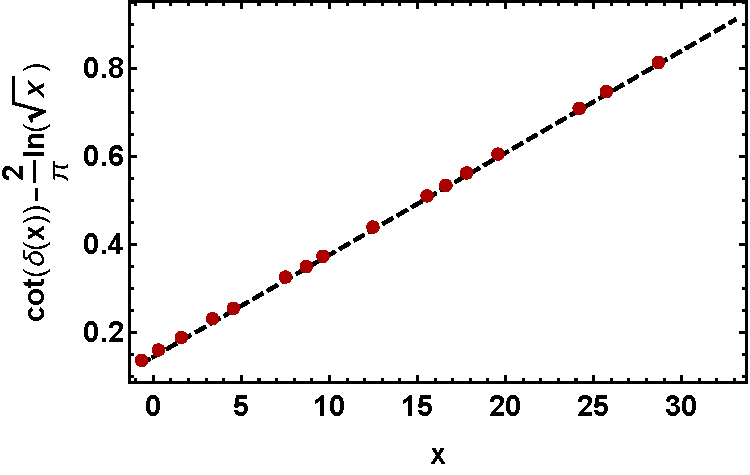
\includegraphics[width=.4925\textwidth]{figure/cotd1.pdf}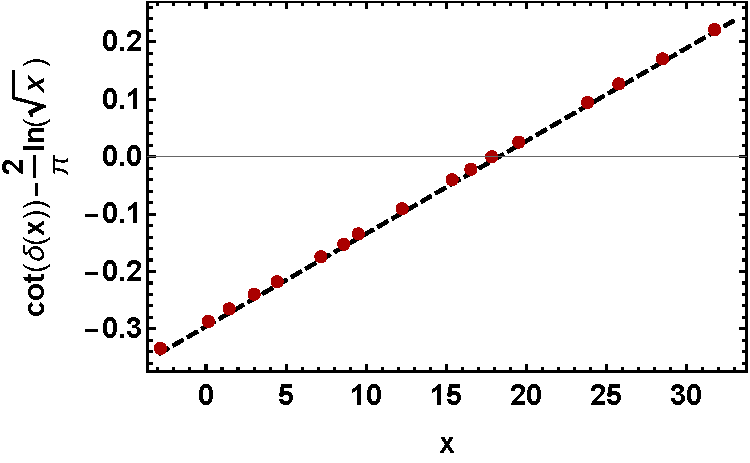
\includegraphics[width=.5075\textwidth]{figure/cotd4.pdf}
\caption{Dashed line is the exact result, the red dots are numerical results.  The potential in this case is given by eq.~\eqref{eqn:potential1}.  Left panel does not support a negative energy solution ($2\pi a_0/L>1$), right panel does ($2\pi a_0/L<1$).\label{fig:cotd1}}
\end{figure}
The agreement between L\"uscher and exact is pretty good.  We have confirmed that as I increase $N$, the points converge to the exact line.  

Our second example uses
\begin{equation}\label{eqn:potential2}
f(p)=\frac{1}{(1+(p/\Lambda)^2)^2}\ .
\end{equation}
Setting
\begin{equation}
\frac{-1}{\mathcal{C}}=\frac{2 \log (a \Lambda )}{\pi }-\frac{11}{6 \pi }\ ,
\end{equation}
we find 
\begin{equation}
\cot \delta(p)=\frac{2 \log (a p)}{\pi }+\frac{p^2 (24 \log (a \Lambda )-13)}{3 \pi  \Lambda ^2}+\frac{p^4 (24 \log (a \Lambda )-19)}{2 \pi  \Lambda
   ^4}
  +\frac{p^6 (8 \log (a \Lambda
   )-7)}{\pi  \Lambda ^6} -\frac{p^8 (11-12 \log (a \Lambda ))}{6 \pi  \Lambda ^8}\ .
\end{equation}
Using the following parameters,
\begin{align*}
a_0&=2 \\
L&=10 \\
N&=100\\
\Lambda&= 5\ ,
\end{align*}
We find good agreement between L\"uscher and the exact result, as shown in the left panel of~\autoref{fig:cotd23}.
\begin{figure}
\center
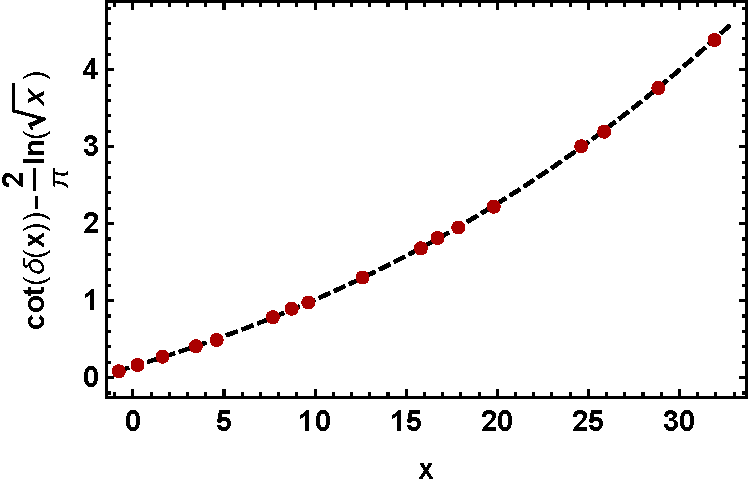
\includegraphics[width=.485\textwidth]{figure/cotd2.pdf}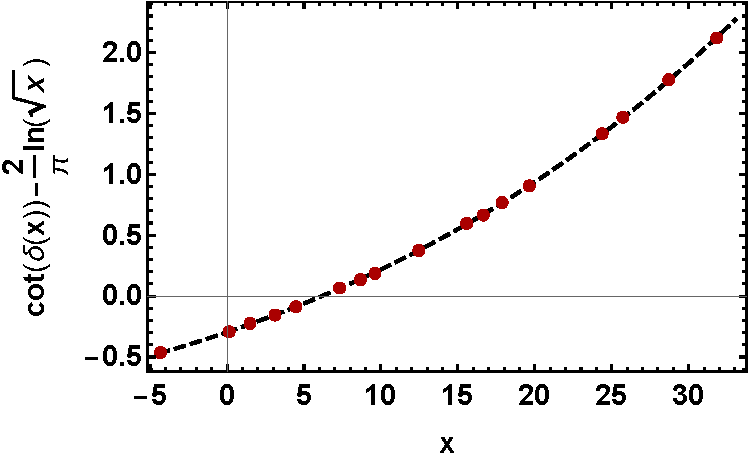
\includegraphics[width=.515\textwidth]{figure/cotd3.pdf}
\caption{Dashed line is the exact result, the red dots are numerical results.  The potential in this case is given by eq.~\eqref{eqn:potential2}.  Left panel does not support a negative energy solution ($2\pi a_0/L>1$), right panel does ($2\pi a_0/L<1$).\label{fig:cotd23}}
\end{figure}
We also reduce the scattering length such that it supports a negative energy solution, $a_0=1$.  The right panel of~\autoref{fig:cotd23} shows this case.  Again, there is good agreement between exact and L\"uscher.